%% BioMed_Central_Tex_Template_v1.06
%%                                      %
%  bmc_article.tex            ver: 1.06 %
%                                       %

%%IMPORTANT: do not delete the first line of this template
%%It must be present to enable the BMC Submission system to
%%recognise this template!!

%%%%%%%%%%%%%%%%%%%%%%%%%%%%%%%%%%%%%%%%%
%%                                     %%
%%  LaTeX template for BioMed Central  %%
%%     journal article submissions     %%
%%                                     %%
%%          <8 June 2012>              %%
%%                                     %%
%%                                     %%
%%%%%%%%%%%%%%%%%%%%%%%%%%%%%%%%%%%%%%%%%


%%%%%%%%%%%%%%%%%%%%%%%%%%%%%%%%%%%%%%%%%%%%%%%%%%%%%%%%%%%%%%%%%%%%%
%%                                                                 %%
%% For instructions on how to fill out this Tex template           %%
%% document please refer to Readme.html and the instructions for   %%
%% authors page on the biomed central website                      %%
%% http://www.biomedcentral.com/info/authors/                      %%
%%                                                                 %%
%% Please do not use \input{...} to include other tex files.       %%
%% Submit your LaTeX manuscript as one .tex document.              %%
%%                                                                 %%
%% All additional figures and files should be attached             %%
%% separately and not embedded in the \TeX\ document itself.       %%
%%                                                                 %%
%% BioMed Central currently use the MikTex distribution of         %%
%% TeX for Windows) of TeX and LaTeX.  This is available from      %%
%% http://www.miktex.org                                           %%
%%                                                                 %%
%%%%%%%%%%%%%%%%%%%%%%%%%%%%%%%%%%%%%%%%%%%%%%%%%%%%%%%%%%%%%%%%%%%%%

%%% additional documentclass options:
%  [doublespacing]
%  [linenumbers]   - put the line numbers on margins

%%% loading packages, author definitions

\documentclass[twocolumn]{bmcart}% uncomment this for twocolumn layout and comment line below
%\documentclass{bmcart}

%%% Load packages
\usepackage{amsthm,amsmath}
\usepackage{siunitx}
\usepackage{mfirstuc}
%\RequirePackage{natbib}
\usepackage[colorinlistoftodos]{todonotes}
\RequirePackage{hyperref}
\usepackage[utf8]{inputenc} %unicode support
%\usepackage[applemac]{inputenc} %applemac support if unicode package fails
%\usepackage[latin1]{inputenc} %UNIX support if unicode package fails
\usepackage[htt]{hyphenat}

\usepackage{array}
\newcolumntype{L}[1]{>{\raggedright\let\newline\\\arraybackslash\hspace{0pt}}p{#1}}

%%%%%%%%%%%%%%%%%%%%%%%%%%%%%%%%%%%%%%%%%%%%%%%%%
%%                                             %%
%%  If you wish to display your graphics for   %%
%%  your own use using includegraphic or       %%
%%  includegraphics, then comment out the      %%
%%  following two lines of code.               %%
%%  NB: These line *must* be included when     %%
%%  submitting to BMC.                         %%
%%  All figure files must be submitted as      %%
%%  separate graphics through the BMC          %%
%%  submission process, not included in the    %%
%%  submitted article.                         %%
%%                                             %%
%%%%%%%%%%%%%%%%%%%%%%%%%%%%%%%%%%%%%%%%%%%%%%%%%


%\def\includegraphic{}
%\def\includegraphics{}

%%% Put your definitions there:
\startlocaldefs
\endlocaldefs


%%% Begin ...
\begin{document}

%%% Start of article front matter
\begin{frontmatter}

\begin{fmbox}
\dochead{Report from 2015 OHBM Hackathon (HI)}

%%%%%%%%%%%%%%%%%%%%%%%%%%%%%%%%%%%%%%%%%%%%%%
%%                                          %%
%% Enter the title of your article here     %%
%%                                          %%
%%%%%%%%%%%%%%%%%%%%%%%%%%%%%%%%%%%%%%%%%%%%%%

\title{LORIS: DICOM Anonymizer}
\vskip2ex
\projectURL{Project URL: \url{http://github.com/aces/DICOM\_anonymizer}}

\author[
addressref={aff1},
corref={aff1},
email={samir@acelab.mcgill.edu.ca}
]{\inits{SD} \fnm{Samir} \snm{Das}}
\author[
addressref={aff2},
%
email={cecile.madjar@gmail.com}
]{\inits{CM} \fnm{C.} \snm{Madjar}}
\author[
addressref={aff3},
%
email={somename@someplace.edu}
]{\inits{AS} \fnm{A.} \snm{Sengupta}}
\author[
addressref={aff1},
%
email={somename@someplace.edu}
]{\inits{ZM} \fnm{Z.} \snm{Mohades}}

%%%%%%%%%%%%%%%%%%%%%%%%%%%%%%%%%%%%%%%%%%%%%%
%%                                          %%
%% Enter the authors' addresses here        %%
%%                                          %%
%% Repeat \address commands as much as      %%
%% required.                                %%
%%                                          %%
%%%%%%%%%%%%%%%%%%%%%%%%%%%%%%%%%%%%%%%%%%%%%%

\address[id=aff1]{%
  \orgname{Montréal Neurological Institute, McGill University and Institute of
Pscychology},
  \city{Montréal},
  \street{1 Queen St},
  \postcode{55332},
  \postcode{Québec},
  \cny{Canada}
}
\address[id=aff2]{%
  \orgname{Douglas Mental Health Institute},
  \city{Montréal},
  \street{2 Queen St},
  \postcode{87777},
  \postcode{Québec},
  \cny{Canada}
}
\address[id=aff3]{%
  \orgname{Otto-von-Guericke University},
  \city{Magdeburg},
  \street{Otto-von-Guericke Strasse 3B},
  \postcode{87777},
  %
  \cny{Germany}
}

%%%%%%%%%%%%%%%%%%%%%%%%%%%%%%%%%%%%%%%%%%%%%%
%%                                          %%
%% Enter short notes here                   %%
%%                                          %%
%% Short notes will be after addresses      %%
%% on first page.                           %%
%%                                          %%
%%%%%%%%%%%%%%%%%%%%%%%%%%%%%%%%%%%%%%%%%%%%%%

\begin{artnotes}
\end{artnotes}

%\end{fmbox}% comment this for two column layout

%%%%%%%%%%%%%%%%%%%%%%%%%%%%%%%%%%%%%%%%%%%%%%
%%                                          %%
%% The Abstract begins here                 %%
%%                                          %%
%% Please refer to the Instructions for     %%
%% authors on http://www.biomedcentral.com  %%
%% and include the section headings         %%
%% accordingly for your article type.       %%
%%                                          %%
%%%%%%%%%%%%%%%%%%%%%%%%%%%%%%%%%%%%%%%%%%%%%%

%\begin{abstractbox}

%\begin{abstract} % abstract
	
%Blank Abstract

%\end{abstract}



%%%%%%%%%%%%%%%%%%%%%%%%%%%%%%%%%%%%%%%%%%%%%%
%%                                          %%
%% The keywords begin here                  %%
%%                                          %%
%% Put each keyword in separate \kwd{}.     %%
%%                                          %%
%%%%%%%%%%%%%%%%%%%%%%%%%%%%%%%%%%%%%%%%%%%%%%

%\vskip1ex

%\projectURL{\url{http://github.com/aces/DICOM\_anonymizer}}
%\projectURL{http://github.com/aces/DICOM\_anonymizer}

% MSC classifications codes, if any
%\begin{keyword}[class=AMS]
%\kwd[Primary ]{}
%\kwd{}
%\kwd[; secondary ]{}
%\end{keyword}

%\end{abstractbox}
%
\end{fmbox}% uncomment this for twcolumn layout

\end{frontmatter}

%{\sffamily\bfseries\fontsize{10}{12}\selectfont Project URL: \url{http://github.com/aces/DICOM\_anonymizer}}

%%% Import the body from pandoc formatted text
\section{Introduction}\label{introduction}

The purpose of this Brainhack project was to create a simple
application, with the least dependencies, for anonymization of DICOM
files directly on a workstation.

Anonymization of DICOM datasets is a requirement before an imaging study
can be uploaded in a web-based database system, such as
LORIS\cite{Das2011}. Currently, a simple and efficient interface for the
anonymization of such imaging datasets, which works on all operating
systems and is very light in terms of dependencies, is not available.

\section{Approach}\label{approach}

Here, we created a DICOM anonymizer that is a simple graphical tool that
uses \href{https://github.com/darcymason/pydicom}{PyDICOM} package to
anonymize DICOM datasets easily on any operating system, with no
dependencies except for the default Python and NumPy packages. DICOM
anonymizer is available for all UNIX systems (including Mac OS) and can
be easily installed on Windows computers as well (see
\href{http://pydicom.readthedocs.org/en/latest/getting_started.html}{PyDICOM
installation}). The GUI (using
\href{https://wiki.python.org/moin/TkInter}{tkinter}) and the processing
pipeline were designed in Python. Executing the anonymizer\_gui.py
script with a python compiler will start the program. Figure 1
illustrates how to use the program to anonymize a DICOM study.

\begin{figure}[h!]
  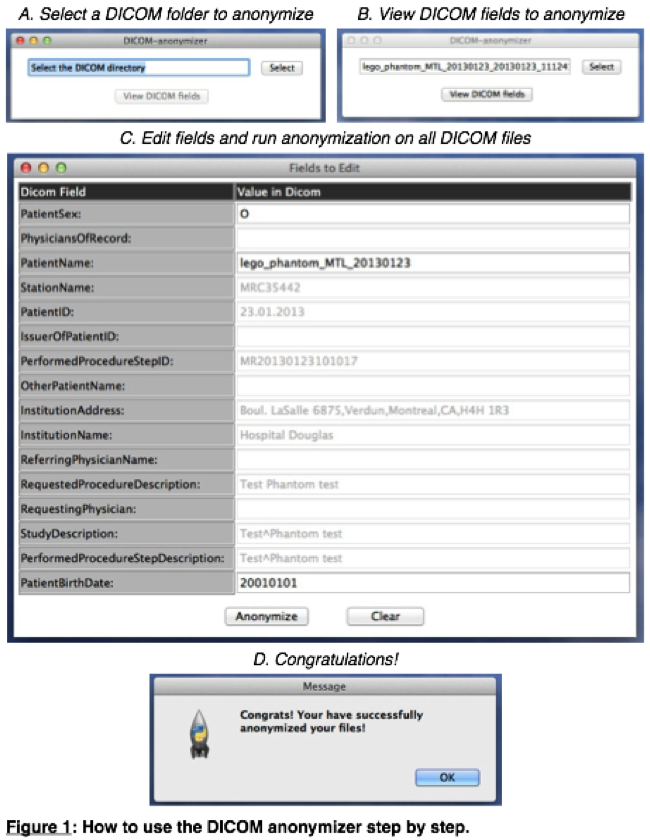
\includegraphics[width=.47\textwidth]{loris_screenshot.png}
  \caption{\label{centfig} How to use the DICOM anonymizer step by step.}
\end{figure}

\section{Results}\label{results}

This graphical tool, designed to be easy-to-use, platform independent
and have minimum dependencies, produces two zip files. One zip file
includes the original DICOM files and the other contains the anonymized
DICOM outputs.

\section{Conclusions}\label{conclusions}

The DICOM anonymizer is a simple standalone graphical tool that
facilitates anonymization of DICOM datasets on any operating system.
These anonymized studies can be uploaded to a web-based database system,
such as LORIS, without compromising the patient or participant's
identity.

%%%%%%%%%%%%%%%%%%%%%%%%%%%%%%%%%%%%%%%%%%%%%%
%%                                          %%
%% Backmatter begins here                   %%
%%                                          %%
%%%%%%%%%%%%%%%%%%%%%%%%%%%%%%%%%%%%%%%%%%%%%%

\begin{backmatter}

\section*{Availability of Supporting Data}
More information about this project can be found at: \url{http://github.com/aces/DICOM\_anonymizer}. Further data and files supporting this project are hosted in the \emph{GigaScience} repository REFXXX.

\section*{Competing interests}
None

\section*{Author's contributions}
SD, CM, AS, and ZM wrote the software and the report.

\section*{Acknowledgements}
The authors would like to thank the organizers and attendees of the 2015
OHBM Hackathon.

  
  
%%%%%%%%%%%%%%%%%%%%%%%%%%%%%%%%%%%%%%%%%%%%%%%%%%%%%%%%%%%%%
%%                  The Bibliography                       %%
%%                                                         %%
%%  Bmc_mathpys.bst  will be used to                       %%
%%  create a .BBL file for submission.                     %%
%%  After submission of the .TEX file,                     %%
%%  you will be prompted to submit your .BBL file.         %%
%%                                                         %%
%%                                                         %%
%%  Note that the displayed Bibliography will not          %%
%%  necessarily be rendered by Latex exactly as specified  %%
%%  in the online Instructions for Authors.                %%
%%                                                         %%
%%%%%%%%%%%%%%%%%%%%%%%%%%%%%%%%%%%%%%%%%%%%%%%%%%%%%%%%%%%%%

% if your bibliography is in bibtex format, use those commands:
\bibliographystyle{bmc-mathphys} % Style BST file
\bibliography{brainhack-report} % Bibliography file (usually '*.bib' )

\end{backmatter}
\end{document}
